\documentclass[12pt]{article}

%useful packages
\usepackage{color,soul}
\usepackage[usenames,dvipsnames,svgnames,table]{xcolor}
\usepackage{amsmath,amsthm,amscd,amssymb,bm}
\usepackage{hyperref}
\hypersetup{
    colorlinks=true,
    linkcolor=JungleGreen
}
\usepackage[utf8]{inputenc}
\usepackage[top=2cm, bottom=3cm, left=2cm, right=2cm]{geometry}
\usepackage{pgfplots}
\usepackage{enumitem}
\usepgfplotslibrary{fillbetween}
\usetikzlibrary{patterns}
\usepackage{tcolorbox}
\usepackage{centernot}
\usepackage{mathtools}
\usepackage{xcolor}

%personal definitions and commands
\newcommand{\R}{\mathbb{R}} 
\newcommand{\E}{\mathbb{E}}
\newcommand{\V}{\mathbb{V}}
\newcommand{\C}{\mathbb{C}}
\newcommand{\Prob}{\mathbb{P}}
\newcommand{\e}{\epsilon}
\newcommand\numberthis{\addtocounter{equation}{1}\tag{\theequation}} %allows numbering of single equations in align* environment
\newcommand{\mtx}[1]{\ensuremath{\bm{\mathit{#1}}}}
\newcommand{\B}{\hat{\boldsymbol{\beta}}}
\newcommand{\Cov}{\mathbb{C}\text{ov}}
\newcommand{\N}{\mathcal{N}}



\title{ECON675: Assignment 2}
\author{Anirudh Yadav}
\setlength\parindent{0pt}
\begin{document}

\maketitle

\setcounter{tocdepth}{2}
\tableofcontents

\newpage

\section{Question 1: Kernel Density Estimation}

\subsection{Density derivatives}
I follow the derivation in Hansen's notes. We are interested in estimating
\begin{align*}
f^{(s)}(x) = \frac{d^s}{dx^s}f(x).
\end{align*}
The natural estimator is
\begin{align*}
\hat f^{(s)}(x)= \frac{d^s}{dx^s}\hat f(x)
\end{align*}
Now, we know that $\hat f(x) = \frac{1}{nh}\sum_i K\left(\frac{X_i - x}{h}\right)$. Thus,
\begin{align*}
\hat f^{(1)}(x) &= \frac{-1}{nh^2}\sum_{i=1}^n K^{(1)}\left(\frac{X_i - x}{h}\right),\\
\hat f^{(2)}(x) &= \frac{1}{nh^3}\sum_{i=1}^n K^{(2)}\left(\frac{X_i - x}{h}\right),\\
&\vdots \\
\hat f^{(s)}(x) &= \frac{(-1)^s}{nh^{1+s}}\sum_{i=1}^n K^{(s)}\left(\frac{X_i - x}{h}\right).
\end{align*}
Now,
\begin{align*}
\E[\hat f^{(s)}(x)] &= \frac{1}{n} \sum_{i=1}^n \E\left[ \frac{(-1)^s}{h^{1+s}}K^{(s)}\left(\frac{X_i - x}{h}\right)\right]\\
&=\E\left[ \frac{(-1)^s}{h^{1+s}}K^{(s)}\left(\frac{X_i - x}{h}\right)\right], \text{ since $X_i$ are iid}.\\
&=\int_{-\infty}^{\infty} \frac{(-1)^s}{h^{1+s}}K^{(s)}\left(\frac{z - x}{h}\right)f(z)dz
\end{align*}
Next, we want to use integration by parts: $\int u dv = uv - \int vdu$. Define
\begin{align*}
dv = \frac{(-1)^s}{h^{s}}\frac{1}{h}K^{(s)}\left(\frac{z - x}{h}\right) \implies v = \frac{(-1)^s}{h^{s}}K^{(s-1)}\left(\frac{z - x}{h}\right)
\end{align*}
And
\begin{align*}
u = f(z) \implies du = f^{(1)}(z).
\end{align*}
Thus,
\begin{align*}
\E[\hat f^{(s)}(x)] &= \left[ \frac{(-1)^s}{h^{s}}K^{(s-1)}\left(\frac{z - x}{h}\right)  f^{(1)}(z)\right]_{-\infty}^{\infty} - \int_{-\infty}^\infty \frac{(-1)^s}{h^{s}}K^{(s-1)}\left(\frac{z - x}{h}\right) f^{(1)}(z)dz.\\
&=- \int_{-\infty}^\infty \frac{(-1)^s}{h^{s}}K^{(s-1)}\left(\frac{z - x}{h}\right) f^{(1)}(z)dz
\end{align*}
Repeating this $s$ times give
\begin{align*}
\E[\hat f^{(s)}(x)] &= (-1)^s \int_{-\infty}^\infty \frac{(-1)^s}{h}K\left(\frac{z - x}{h}\right) f^{(s)}(z)dz\\
&=\int_{-\infty}^\infty \frac{1}{h}K\left(\frac{z - x}{h}\right) f^{(s)}(z)dz
\end{align*}
Next, use the following change of variables: $u = \frac{z - x}{h}$, which implies $z = x + hu \implies dz = hdu$. Thus,
\begin{align}
\E[\hat f^{(s)}(x)] &= \int_{-\infty}^\infty K(u) f^{(s)}(x+hu)du \label{eq:der1}
\end{align}
The next step is to take a Taylor expansion of $f^{(s)}(x+hu)$ around $x+hu = x$, which is valid if $h \to 0$. We get
\begin{align*}
f^{(s)}(x+hu) = f^{(s)}(x) + f^{(s+1)}(x)hu + \frac{1}{2}f^{(s+2)}(x)h^2u^2 + ... + \frac{1}{P!} f^{(s+P)}(x)h^Pu^P + o(h^P).
\end{align*}
Substituting this expression back into (\ref{eq:der1}), integrating over each term, and using the fact that $\int_{-\infty}^\infty K(u)du = 1$ and the notation
\begin{align*}
\mu_\ell(K) = u^\ell K(u)
\end{align*}
gives
\begin{align*}
\E[\hat f^{(s)}(x)] &= f^{(s)}(x) + f^{(s+1)}(x)h\mu_1(K) + \frac{1}{2}f^{(s+2)}(x)h^2\mu_2(K) + ... + \frac{1}{P!} f^{(s+P)}(x)h^P\mu_P(K) + o(h^P).
\end{align*}
Finally, noting that since $K$ is a $P$-order kernel, $\mu_\ell(K) = 0$ for all $\ell < P$, gives the desired result
\begin{align}
\E[\hat f^{(s)}(x)] &= f^{(s)}(x) + \frac{1}{P!} f^{(s+P)}(x)h^P\mu_P(K) + o(h^P). \label{eq:der2}
\end{align}

Next we consider the variance of the derivative estimator.
\begin{align*}
\V[\hat f^{(s)}(x)] &= \V\left[\frac{(-1)^s}{nh^{1+s}}\sum_{i=1}^n K^{(s)}\left(\frac{X_i - x}{h}\right)\right]\\
&=\frac{1}{nh^{2+2s}}\V\left[K^{(s)}\left(\frac{X_i - x}{h}\right)\right],
\end{align*}
since $\{X_i\}$ are iid there are no covariance terms and each term has the same variance. Continuing,
\begin{align}
\V[\hat f^{(s)}(x)] &=\frac{1}{nh^{2+2s}} \left\{\E\left[K^{(s)}\left(\frac{X_i - x}{h}\right)^2\right] - \E\left[K^{(s)}\left(\frac{X_i - x}{h}\right)\right]^2 \right\} \nonumber \\
&=\frac{1}{nh^{2+2s}} \E\left[K^{(s)}\left(\frac{X_i - x}{h}\right)^2\right] - \frac{1}{n} \E\left[\frac{1}{h^{1+s}}K^{(s)}\left(\frac{X_i - x}{h}\right)\right]^2 \label{eq:der3}
\end{align}
Now, from above we know that
\begin{align*}
\E\left[\frac{1}{h^{1+s}}K^{(s)}\left(\frac{X_i - x}{h}\right)\right] & =  f^{(s)}(x) + \frac{1}{P!} f^{(s+P)}(x)h^P\mu_P(K) + o(h^P)\\
&= f^{(s)}(x) + o(1)
\end{align*}
since the remainder goes to zero as $h\to0$. Thus, the second term in (\ref{eq:der3}) is $O(\frac{1}{n})$; i.e. the same order as $1/n$. Furthermore $O(\frac{1}{n})$ is of smaller order than $O(\frac{1}{nh^{1+2s}})$ since $h \to 0$ and $n\to \infty$. Accordingly, we can write
\begin{align*}
\V[\hat f^{(s)}(x)] &=\frac{1}{nh^{2+2s}} \E\left[K^{(s)}\left(\frac{X_i - x}{h}\right)^2\right] + o\left(\frac{1}{nh^{1+2s}}\right),
\end{align*}
Thus,
\begin{align*}
\V[\hat f^{(s)}(x)] &=\frac{1}{nh^{1+2s}} \int_{-\infty}^{\infty}\frac{1}{h}K^{(s)}\left(\frac{z- x}{h}\right)^2 f(z) dz + o\left(\frac{1}{nh^{1+2s}}\right)
\end{align*}
Again we use the change of variables $u = \frac{z - x}{h}$ so that
\begin{align*}
\V[\hat f^{(s)}(x)] &=\frac{1}{nh^{1+2s}} \int_{-\infty}^{\infty}K^{(s)}(u)^2 f(x+hu) du + o\left(\frac{1}{nh^{1+2s}}\right)
\end{align*}
With the usual Taylor expansion of $f(x+hu)$ we can write
\begin{align*}
\V[\hat f^{(s)}(x)] &=\frac{1}{nh^{1+2s}} \int_{-\infty}^{\infty}K^{(s)}(u)^2 (f(x) + O(h)) du + o\left(\frac{1}{nh^{1+2s}}\right)\\
&=\frac{f(x)}{nh^{1+2s}} \int_{-\infty}^{\infty}K^{(s)}(u)^2 du + o\left(\frac{1}{nh^{1+2s}}\right)\\
&=\frac{1}{nh^{1+2s}}f(x)\vartheta_{s}(K) + o\left(\frac{1}{nh^{1+2s}}\right),
\end{align*}
where $\vartheta_{s}(K) =  \int_{-\infty}^{\infty}K^{(s)}(u)^2 du$ as required.

\newpage

\subsection{Optimal bandwidth}
We have
\begin{align*}
\text{AIMSE} [h] &= \int_{-\infty}^{\infty} \left[\left(h^P \mu_P(K) \cdot \frac{f^{(P+s)}(x)}{P!}\right)^2+\frac{1}{nh^{1+2s}}\vartheta_s(K)f(x)\right]dx\\
&= h^{2P}\left(\frac{\mu_P(K)}{P!}\right)^2\vartheta_{s+P}(f) + \frac{1}{nh^{1+2s}}\vartheta_s(K),
\end{align*}
since $f(x)$ integrates to 1 and where $\vartheta_{s+P}(f) = \int (f^{(P+s)}(x))^2dx$. Thus,
\begin{align*}
\frac{d}{dh}\text{AIMSE} [h] = 2Ph^{2P-1}\left(\frac{\mu_P(K)}{P!}\right)^2\vartheta_{s+P}(f) - (1+2s)\frac{1}{nh^{2+2s}}\vartheta_s(K)&=0\\
\implies 2Ph^{1+2P+2s}\left(\frac{\mu_P(K)}{P!}\right)^2\vartheta_{s+P}(f)  &=(1+2s)\frac{1}{n}\vartheta_s(K),
\end{align*}
which gives the optimal bandwidth
\begin{align*}
h^* = \left[\frac{1+2s}{2Pn}\left(\frac{P!}{\mu_P(K)}\right)^2\frac{\vartheta_s(K)}{\vartheta_{s+P}(f)}\right]^{\frac{1}{1+2P+2s}}.
\end{align*}
A fully data-driven method for estimating $h^*$ is cross-validation. This procedure attempts to directly estimate the mean-squared error, and then choose the bandwidth which minimizes this estimate. From the lecture notes the cross-validation bandwidth is the value $h$ which minimizes the criteria
\begin{align*}
\hat h_{CV} = \arg \min_{h} CV(h) &= \frac{1}{n^2h} \sum_{i=1}^n \sum_{j=1}^n (K*K) \left(\frac{X_i - X_j}{h}\right) - \frac{2}{n}\sum_{i=1}^n \hat f_{(i)}(X_i)
\end{align*}
where $ \hat f_{(i)}(x_i)$ is the density estimate computed without observation $X_i$.

\subsection{Monte Carlo experiment}

\textbf{(a)} First, we want to compute the theoretically optimal bandwidth for $s=0$, $n=1000$, using the Epanechnikov kernel $(P=2)$, with the following Gaussian DGP:
\begin{align*}
x_i \sim 0.5 \N(-1.5,-1.5) + 0.5\N(1,1)
\end{align*}
From Table 1 in Hansen's notes, $\mu_2(K)=1/5$ and $\vartheta(K)=3/5$ for the Epanechnikov kernel. Thus, the only other ingredient we need is $\vartheta_{2}(f) = \int [f^{(2)}(x)]^2 dx$ for the above DGP. Note that the second derivative of the normal density with mean $\mu$ and variance $\sigma^2$ is
\begin{align*}
\phi^{(2)}_{\mu, \sigma^2}(x) = \frac{1}{\sqrt{2\pi \sigma^2}}\exp\left(-\frac{(x-\mu)^2}{\sigma^2}\right)\left[\left(\frac{x-\mu}{\sigma^2}\right)^2 - \frac{1}{\sigma^2}\right]
\end{align*}
Since differentiation is a linear operation, we have
\begin{align*}
\vartheta_{2}(f) = \int_{-\infty}^\infty [0.5\times\phi^{(2)}_{-1.5, 1.5}(x) + 0.5\times \phi^{(2)}_{1, 1}(x)]^2 dx \approx 0.0388.
\end{align*}
Finally, we get the theoretically optimal bandwidth
\begin{align*}
h^* = \left[\frac{1}{2 \times 2 \times 1000}\left(\frac{2!}{1/5}\right)^2\frac{3/5}{\vartheta_{2}(f)}\right]^{\frac{1}{1+2\times 2}} \approx 0.827.
\end{align*}

\textbf{(b)} I plot the IMSE estimates for the full-sample and leave-one-out sample below (see Appendix for the code).

\begin{figure}[h]
    \centering
    
        %\centering
        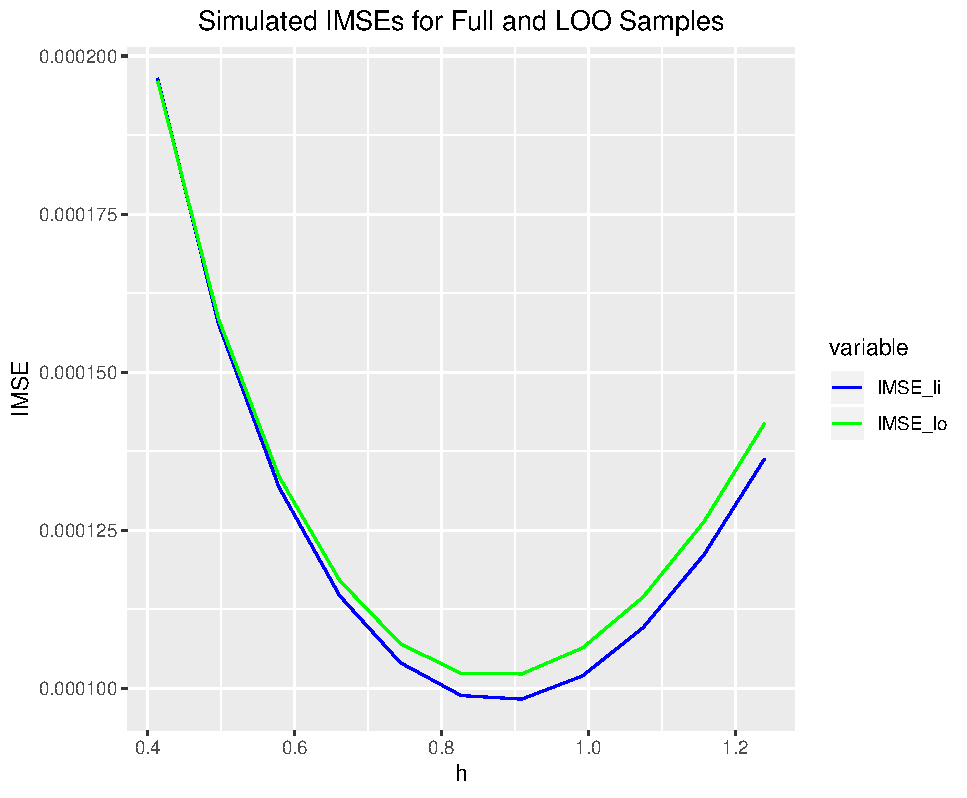
\includegraphics[width=0.8\textwidth]{Q1_IMSE.pdf}
        \caption{Estimated IMSE for $M=1000$ simulations.}

\end{figure}

\textbf{(c)} Somewhat strangely, I find that $h_{\widehat{IMSE,LI}}=h_{\widehat{IMSE,LO}} = 1.1 \times h^*$. I suppose as we increase $M$, the estimates should converge to $h^*$.\\

\textbf{(d)} I get the following rule-of-thumb bandwidth
\begin{align*}
\bar{h}_{\texttt{AIMSE}} = \frac{1}{M} \sum_{i=1}^M \hat{h}_{\texttt{AIMSE},m} \approx 0.985,
\end{align*}
which is about $1.2 \times h^*$.

\newpage

\section{Linear smoothers, cross-validation and series}

\subsection{Local polynomial and series estimation as linear smoothers} We are interested in estimating the regression function $e(x) = \E[y_i | x_i = x]$. The idea of local polynomial regression is to approximate $e(x)$ locally by a polynomial of degree $p$, and estimate this local approximation by weighted least squares. For each $x$ we solve
\begin{align*}
\hat{\mtx{\beta}}(x) &= \arg \min_{\beta \in \R^{p+1}}\sum_{i=1}^n[y_i - \beta_0 - \beta_1(x_i-x) - \beta_2(x_i-x)^2 -...-\beta_p(x_i-x)^p]^2K\left(\frac{x_i - x}{h}\right).
\end{align*}
where
\begin{align*}
\hat e(x) = \hat \beta_0
\end{align*}
Note that this is motivated by a Taylor expansion of the true regression function $e(x_i)$ around $x$. And note that the kernel is just a `smooth' way of weighting observations that are close to the evaluation point $x$.\\

More compactly, we write
\begin{align*}
\hat{\mtx{\beta}}_{\texttt{LP}}(x)  = \arg \min_{\beta \in \R^{p+1}}\sum_{i=1}^n [y_i - \mtx{r}_p(x_i - x)'\mtx{\beta}]^2K\left(\frac{x_i - x}{h}\right)
\end{align*}
where $\mtx{r}_p(u)= (1 , u , u^2 ,...,u^p)'$. \\

From the lecture notes, we know that
\begin{align*}
\hat{\mtx{\beta}}_{\texttt{LP}}(x)  = (\mtx{R}'_p \mtx{W} \mtx{R}_p)^{-1}\mtx{R}'_p \mtx{W} \mtx{y}
\end{align*}
where
\begin{align*}
\mtx{R}_p = 
\begin{bmatrix}
1 & (x_1 - x) & (x_1-x)^2 & \dots& (x_1-x)^p \\
1 & (x_2 - x) & (x_2-x)^2 & \dots &(x_2-x)^p\\
\vdots & \vdots & \dots & \ddots & \vdots \\
1 & (x_n - x) & (x_n-x)^2 & \dots &(x_n-x)^p
\end{bmatrix}
\end{align*}
and $\mtx{W} = \text{diag}\left(K\left(\frac{x_1 - x}{h}\right), K\left(\frac{x_2 - x}{h}\right),..., K\left(\frac{x_n - x}{h}\right) \right)$.\\

Then
\begin{align*}
\hat{\mtx{e}}(x) &= \mtx{e}_1'\hat{\mtx{\beta}}_{\texttt{LP}}(x)  \\
&=\mtx{e}_1'(\mtx{R}'_p \mtx{W} \mtx{R}_p)^{-1}\mtx{R}'_p \mtx{W} \mtx{y}
\end{align*}
where $ \mtx{e}_1$ the first standard basis vector of length $(1+p)$ (i.e. it has a 1 in the first entry and zeros in the remaining $p$ entries). I think in summation form we can write
\begin{align*}
\hat{\mtx{e}}(x) &= \mtx{e}_1' (\sum_{i=1}^n \mtx{r}_p(x_i-x)\mtx{r}_p(x_i-x)' w_i)^{-1}(\sum_{i=1}^n \mtx{r}_p(x_i-x)w_iy_i)
\end{align*}
where $w_i = K\left(\frac{x_i - x}{h}\right)$.\\

Next we consider series estimation of the regression function $e(x)$. A series approximation to $e(x)$ is a global approximation, unlike the local polynomial regression. A series approximation that uses a polynomial basis (c.f. splines) takes the form
\begin{align*}
\hat{\mtx{\beta}}_{\texttt{Series}} = \arg \min_{\beta \in \R^{p+1}} \sum_{i=1}^n (y_i - \mtx{r}_p(x_i)' \mtx{\beta})^2
\end{align*}
where $\mtx{r}_p(x_i) = (1, x_i, x_i^2, ..., x_i^p)$. And
\begin{align*}
\hat e(x) =  \mtx{r}_p(x)'\hat{\mtx{\beta}}_{\texttt{Series}} 
\end{align*} 

Accordingly, we have
\begin{align*}
\hat{\mtx{\beta}}_{\texttt{Series}} = \left(\mtx{R}'_p \mtx{R}_p \right)^{-1} \mtx{R}_p \mtx{y}
\end{align*}
where
\begin{align*}
\mtx{R}_p = 
\begin{bmatrix}
1 & (x_1) & (x_1)^2 & \dots& (x_1)^p \\
1 & (x_2) & (x_2)^2 & \dots &(x_2)^p\\
\vdots & \vdots & \dots & \ddots & \vdots \\
1 & (x_n) & (x_n)^2 & \dots &(x_n)^p
\end{bmatrix}
\end{align*}
And,
\begin{align*}
\hat e(x) =  \mtx{r}_p(x)' \left(\mtx{R}'_p \mtx{R}_p \right)^{-1} \mtx{R}_p \mtx{y},
\end{align*}
which is of the linear smoother form. In summation form
\begin{align*}
\hat e(x) =  \mtx{r}_p(x)' (\sum_{i=1}^n  \mtx{r}_p(x_i) \mtx{r}_p(x_i)')^{-1} (\sum_{i=1}^n  \mtx{r}_p(x_i) y_i).
\end{align*}

\subsection{Cross validation}
The idea of cross-validation is to choose the tuning parameter (e.g. bandwidth, etc.) that minimizes the mean squared leave-one-out error
\begin{align*}
\hat c = \arg \min_c \frac{1}{n} \sum_{i=1}^n (y_i - \hat e_{(i)}(x_i; c))^2
\end{align*}
where $\hat e_{(i)}(x_i)$ is the estimator of the regression function that ``leaves out'' $x_i$.\\ 

From the above results we know that both the local polynomial and series estimators can be written as
\begin{align*}
\hat{\mtx{e}}(x) = \mtx{S}\mtx{y}
\end{align*}
where $\mtx{S}$ is the `smoothing' matrix. Note that for local polynomial and series estimators the smoothing matrix is constant preserving in the sense $\mtx{S}{\mtx{1}} = \mtx{1}$. That is, the rows of \mtx{S} sum to one. In leave-one-out cross validation, we want to use the same smoother with the $i$-th row and column deleted; we also want this to be an $(n -1) \times (n - 1)$ smoother matrix. Accordingly, we must renormalize the rows to sum to one. Let $w_{ij}$ denote the elements of $\mtx{S}$. When we delete the $i$-th column, then the $i$-th row now sums to $1- w_{ii}$. So, we divide by $1- w_{ii}$ to renormalize. Accordingly, the leave-one-out estimator is
\begin{align*}
\hat e_{(i)}(x_i) = \frac{1}{1-w_{ii}} \sum_{j=1,j\neq i}^n w_{ij}y_i
\end{align*}
And note that the full-sample estimator is just
\begin{align*}
\hat e(x_i) = \sum_{j=1}^n w_{ij}y_i.
\end{align*}
From the above expression we get
\begin{align*}
\hat e_{(i)}(x_i)(1-w_{ii}) &=\sum_{j=1,j\neq i}^n w_{ij}y_i\\
\hat e_{(i)}(x_i) &= \sum_{j=1,j\neq i}^n w_{ij}y_i + w_{ii}\hat e_{(i)}(x_i)\\
&=\sum_{j=1}^n w_{ij}y_i + w_{ii}\hat e_{(i)}(x_i) - w_{ii}y_i\\
&=\hat e(x_i)  + w_{ii}\hat e_{(i)}(x_i) - w_{ii}y_i\\
\implies y_i - \hat e_{(i)}(x_i) &= y_i -\hat e(x_i)  - w_{ii}\hat e_{(i)}(x_i) + w_{ii}y_i\\
&=y_i - \hat e(x_i) + w_{ii}(y_i - \hat e_{(i)}(x_i))\\
\therefore y_i - \hat e_{(i)}(x_i) &= \frac{1}{1-w_{ii}}(y_i - \hat e(x_i)),
\end{align*}
which gives the desired result.

\subsection{Asymptotic distribution}
First note that we have iid data. Also note that we must have $\sum_{i=1}^n w_{n,i}(x_i) = 1$. To ease notation, denote $\E[\cdot | x_1, x_2,...,x_n; x]$ as $\E[\cdot| x]$. Then
\begin{align*}
\E[\hat e(x)|x] &= \E[\sum_{i=1}^n w_{n,i}(x_i)y_i|x]\\
&=\sum_{i=1}^n\E[ w_{n,i}(x_i)y_i|x]\\
&=\sum_{i=1}^nw_{n,i}(x_i)\E[y_i|x]\\
&=\E[y_i|x].
\end{align*}
Thus, so long as $\hat e(x)$ has a finite second moment we can use the classical CLT to get asymptotic normality. Now, 
\begin{align*}
\V[\hat e(x) | x] &= \V[\sum_{i=1}^n w_{n,i}(x)y_i|x]\\
&=\sum_{i=1}^n\V[w_{n,i}(x)y_i|x]\\
&=\V[y_i|x]\sum_{i=1}^nw_{n,i}(x)^2\\
\end{align*}
Then we get the consistent variance estimator
\begin{align*}
\hat{V}(x) = \hat{\sigma}^2  \sum_{i=1}^nw_{n,i}(x)^2
\end{align*}
where $\hat{\sigma}^2 = \frac{1}{n-1}\sum_{i=1}^n (y_i - \hat e(x_i))^2$


\subsection{Confidence intervals}
The pointwise asymptotically valid 95\% CI for $e(x)$ is
\begin{align*}
CI_{95}(x) = [ \hat e(x) - 1.96 \sqrt{\hat{V}(x)},\hat e(x) + 1.96\cdot \sqrt{\hat{V}(x)}].
\end{align*}
This is clearly different to a confidence band that is uniformly valid over all $x$. Uniform confidence bands would be specified as
 \begin{align*}
\sup_{x \in \chi}\left|\frac{\hat e(x) - e(x)}{\sqrt{\hat\V(x)}} \right| \leq q_{1-\alpha/2},
\end{align*}
which is clearly a harder problem than the pointwise intervals.

\subsection{Monte Carlo experiment}

\textbf{(a)} See attached code.\\

\textbf{(b)} I plot the average CV(K), across the $M=1000$ simulations below. 

\begin{figure}[h!]
    \centering
    
        %\centering
        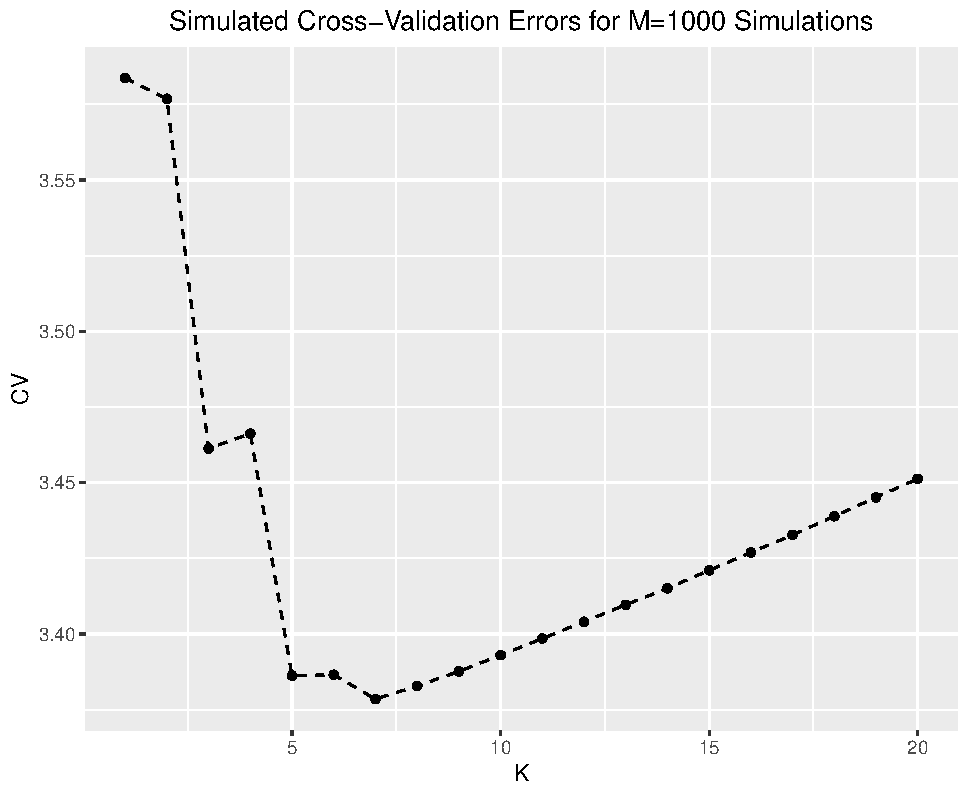
\includegraphics[width=0.7\textwidth]{Q2_CV.pdf}
        \caption{Estimated CV error for $M=1000$ simulations.}

\end{figure}
\newpage

Accordingly, the cross validation polynomial order is $\hat K_{CV} = 7 $.\\

\textbf{(c)} I plot the true regression function and the series estimate below.

\begin{figure}[h!]
    \centering
    
        %\centering
        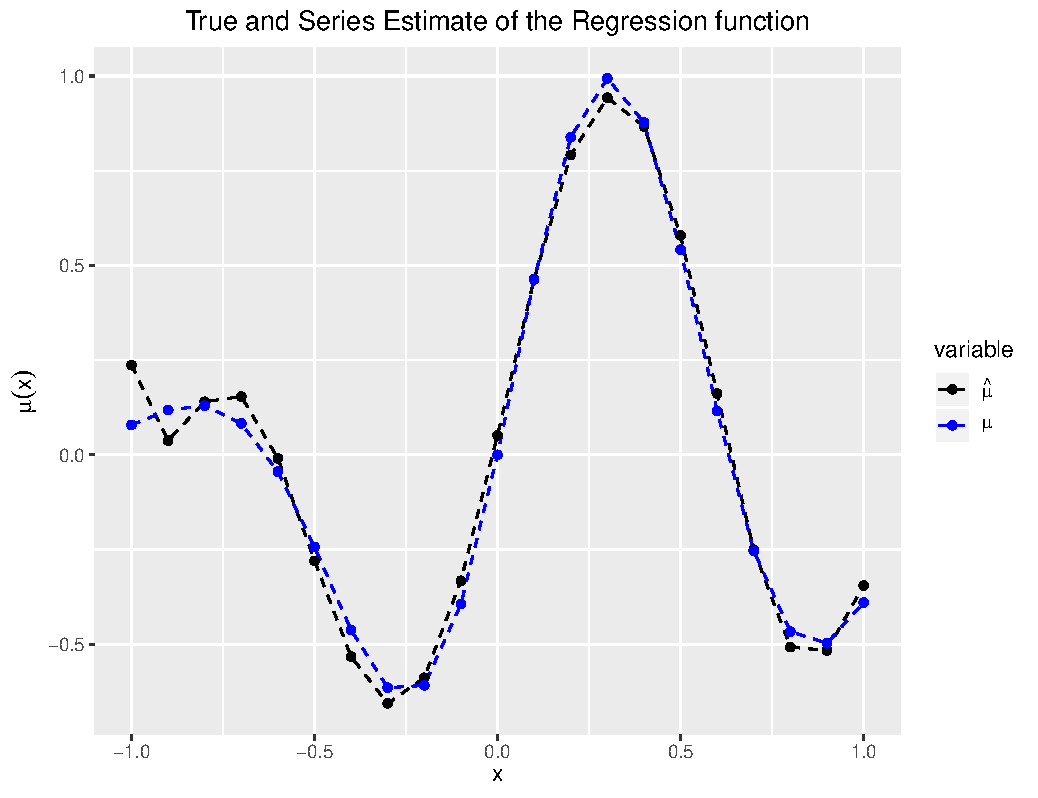
\includegraphics[width=0.7\textwidth]{Q2_diag.pdf}
        %\caption{}
\end{figure}

\textbf{(d)} Next we want to estimate the derivative of the true regression function. I shall assume that $\hat K_{CV}=7$ is also the optimal order for the series estimate of $\mu^{(1)}(x)$. Now, the derivative of the true regression function is
\begin{align*}
\frac{d}{dx}\mu(x) = \exp(-0.1(4x-1)^2)\left[5 \cos(5x) - 0.8 (4x-1)\sin(5x)\right].
\end{align*}
And the series estimate of the derivative is simply the derivative of the original series estimate:
\begin{align*}
\widehat{\frac{d}{dx}\mu(x)}&=\frac{d}{dx}\hat \mu(x)\\
&=(0,1,2x,3x^2,4x^3,5x^4,6x^5,7x^6) \cdot \hat{\beta}_{CV}
\end{align*}
I plot the true derivative and the series estimate below.

\begin{figure}[h!]
    \centering
    
        %\centering
        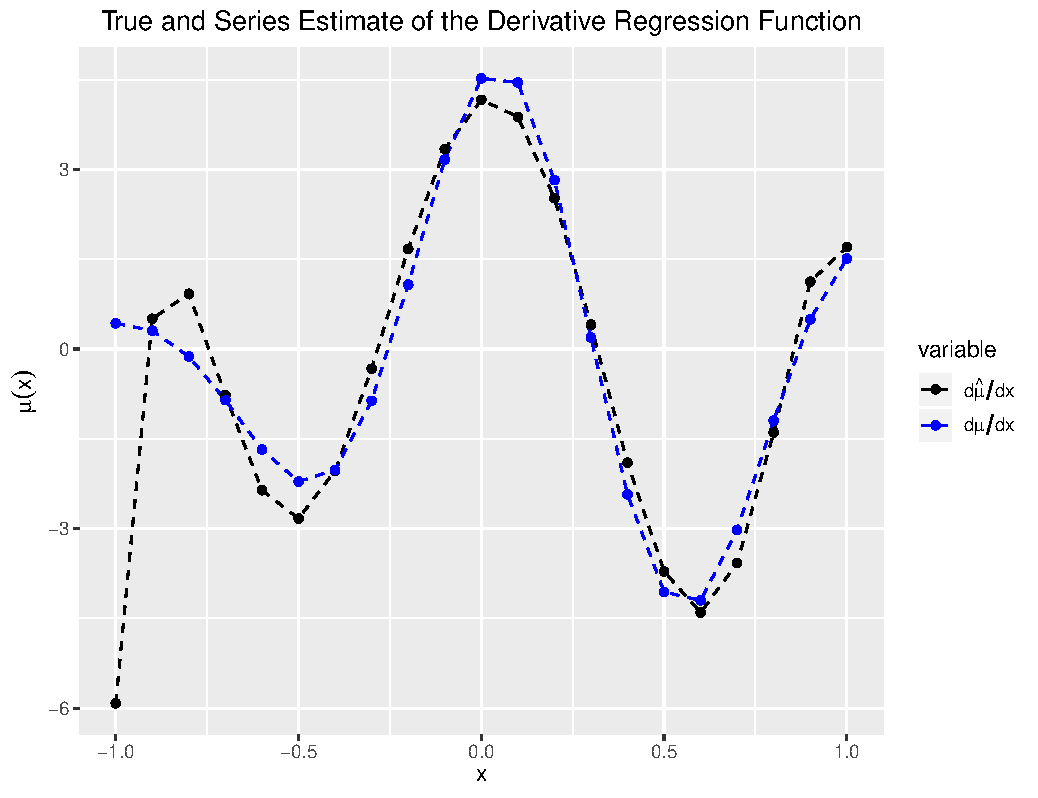
\includegraphics[width=0.7\textwidth]{Q2_diagder.pdf}
        %\caption{}
\end{figure}



\newpage

\section{Semiparametric semi-linear model}
We have the partially linear model
\begin{align}
y_i = t_i \theta_0 + g_0(\mtx{x_i}) + \e_i, \label{eq:3a}
\end{align}
with the usual heteroskedasticity assumptions for the error.
\subsection{}
From Li-Racine 7.1.1 (p 222) we know that for $\theta_0$ to be identifiable, $t_i$ must not contain a constant (since $t_i$ is a treatment dummy, this is clearly satisfied) or any deterministic functions of $\mtx{x}_i$. 

Now, somehow we need to show
\begin{align*}
\E[(t_i-h_0(\mtx{x}_i))(y_i - t_i\theta_0)]&=0
\end{align*}
Then we have
\begin{align*}
\E[y_i (t_i-h_0(\mtx{x}_i))- t_i\theta_0(t_i-h_0(\mtx{x}_i))]&=0\\
\E[t_i\theta_0(t_i-h_0(\mtx{x}_i))] &= \E[y_i (t_i-h_0(\mtx{x}_i))]\\
\therefore \theta_0 &= \E[t_i(t_i-h_0(\mtx{x}_i))]^{-1}\E[y_i (t_i-h_0(\mtx{x}_i))].
\end{align*}
The IV interpretation is that we are using $t_i-h_0(\mtx{x}_i)$ as an instrument for $t_i$.

\subsection{Series estimation}
\textbf{(a)} Consider the power series approximation
\begin{align*}
\E[y_i |\mtx{x}_i] \approx t_i \theta_0 + \mtx{p}^K(\mtx{x}_i)'\mtx{\gamma}_K.
\end{align*}
Using the usual partition regression formula we get the OLS estimator
\begin{align*}
\hat \theta(K) = (\mtx{t}'\mtx{M}_{X}\mtx{t})^{-1}\mtx{t}'\mtx{M}_X\mtx{Y}
\end{align*}
where $\mtx{t} = (t_1, ...,t_n)'$ and 
\begin{align*}
\mtx{M}_X = \mtx{I} - \mtx{P}_X
\end{align*}
and
\begin{align*}
\mtx{P}_X =\mtx{R}_p \left(\mtx{R}'_p \mtx{R}_p \right)^{-1} \mtx{R}'_p \
\end{align*}
\begin{align*}
\mtx{R}_p = 
\begin{bmatrix}
1 & (\mtx{x}_1) & (\mtx{x}_1)^2 & \dots& (\mtx{x}_1)^p \\
1 & (\mtx{x}_2) & (\mtx{x}_2)^2 & \dots& (\mtx{x}_2)^p\\
\vdots & \vdots & \dots & \ddots & \vdots \\
1 & (\mtx{x}_n) & (\mtx{x}_n)^2 & \dots& (\mtx{x}_n)^p
\end{bmatrix}
\end{align*}

\textbf{(b)}
We have the moment condition
\begin{align*}
\theta_0 &= \E[t_i(t_i-h_0(\mtx{x}_i))]^{-1}\E[y_i (t_i-h_0(\mtx{x}_i))]
\end{align*}
The M-estimator is simply
\begin{align*}
\hat \theta_M &=\left(\frac{1}{n}\sum_{i=1}^nt_i(t_i-\hat h(\mtx{x}_i))\right)^{-1} \left(\frac{1}{n}\sum_{i=1}^n y_i (t_i-\hat h(\mtx{x}_i))\right)\\
&=\left(\sum_{i=1}^nt_i(t_i- \hat h(\mtx{x}_i))\right)^{-1} \left(\sum_{i=1}^n y_i (t_i- \hat h(\mtx{x}_i))\right).
\end{align*}
where $\hat h(\mtx{x}_i)$ is the estimated propensity score (could be estimated by logit/probit, etc.)

\subsection{Asymptotics}
\textbf{(a)}\\

\textbf{(b)}



\end{document}
